% ==============================
\section{lezione del 20-03-26}
\subsection{Variabili aleatorie binomiali}\label{sub:Variabili aleatorie binomiali} % (fold)
Si ripeta $N$ volte un esperimento aleatorio nel quale un certo evento $A$ si presenta
con probabilità $p$ in ciascuna prova (le prove sono \textit{indipendenti}).
Possiamo definire una v.a. $X$ il cui valore di indentifica sul numero totale delle volte
che l'evento $A$ si verifica sul totale delle $N$ prove. Tale v.a. detta \textit{numero di successi} è di 
tipo discreto e può assumere valori $x_k = 1,2, \dots, N$ con massa di probabiltà:
\[
    p_X(k) = p(\{X = k\}) = \binom{N}{k}p^k(1 - p)^{N-k}, \quad 0 < p < 1,\quad k = 0, 1, \dots, N
\]
\begin{definition}\label{variabile aleatorio binomiale}
    Una varibile aleatoria $X \in B(p, N)$ è detta binomiale se è discreta 
    definita per valori interi $0, 1, 2, \dots, N$  con la seguente massa di probabità
    \begin{displaymath}
                p_X(k) = p(\{X = k\}) = \binom{N}{k}p^k(1 - p)^{N-k}, \quad 0 < p < 1,\quad k = 0, 1, \dots, N 
    \end{displaymath}
\end{definition}
% subsection Variabili aleatorie binomiali (end)
\subsection{Varibili aleatorie di Poisson}\label{sub:Varibili aleatorie di Poisson} % (fold)
Diamo subito la definizione
\begin{definition}\label{variabile aleatorio di Poisson}
    Una variabile aleatori $X \in P(\Lambda)$ è detta di \textbf{Poisson} di paramentro $\Lambda$ con $\Lambda > 0$ 
    se è discreta, definita per valori positivi e ha la seguente massa di probabiltà
    \begin{displaymath}
        P_X(k) =P(\{X = k\}) = \frac{\Lambda^k}{k!}e^{-\Lambda}, \quad k = 1, 2, \dots 
    \end{displaymath}
\end{definition}
Notiamo che vale la \textit{condizione di normalizzazione}
\[
    \sum_{k = 0}^{+\infty}p_X(k) = e^{-\Lambda} \sum_{k = 0}^{+\infty}\frac{\Lambda^k}{k!} = e^{-\Lambda}e^{\Lambda} = 1
\]
% subsection Varibili aleatorie di Poisson (end)
\subsubsection{Decadimento Radioattivo}\label{sec:Decadimento Radioattivo} % (fold)
Supponiamo di studiare una sostanza radioattiva a vita media molto lunga
(in modo da poter considerare costante l’intensità radioattiva per tutta la
durata dell’osservazione). Il numero di decadimenti per unità di tempo è schematizzabile come una
variabile aleatoria di Poisson di parametro $\Lambda = 0.5$ decadimenti al secondo
\begin{importantbox}
    \textit{Calcolare la probabilità che l’intervallo di tempo intercorrente fra due
    decadimenti successivi superi un secondo}
\end{importantbox}
Notiamo subito che se  $F_X(x)$ di una v.a. discreta
è nota, è possibile dedurre sia i valori assunti dalla v.a., sia le
corrispondenti probabilità quindi dalla $F_X(x)$ possiamo ricavare la massa di probabilità
\[
    F_X(x) = P(\{hX \leq x\}) = \sum_{\{i: x_i \leq x\}} P(\{X = x_1\}) = \sum_{\{i: x_i \leq x\}} p_X(x_i)
\]
\[
    = \sum_i P(\{X = x_i\})u(x - x_i) = \sum_i p_X(x_i)u(x - x_i)
\]

\begin{center}
\begin{tikzpicture}

% --- GRAFICO A) PMF ---
\begin{axis}[
    name=plotA,
    width=10cm, height=5cm,
    axis lines=middle,
    xlabel={$x$}, ylabel={$p_i$},
    xmin=0, xmax=6,
    ymin=0, ymax=0.35,
    xtick={1, 2, 3, 4, 5},
    xticklabels={$x_1$, $x_2$, $x_3$, $x_4$, $x_5$},
    ytick={0.1, 0.2, 0.3},
    every axis x label/.style={at={(current axis.right of origin)}, anchor=west},
    every axis y label/.style={at={(current axis.north)}, anchor=south},
    title style={at={(0,1)}, anchor=north west},
    title={\textbf{a)}}
]
    \addplot[ycomb, thick, mark=none] coordinates {
        (1, 0.15) (2, 0.25) (3, 0.1) (4, 0.2) (5, 0.3)
    };
\end{axis}

% --- GRAFICO B) CDF ---
\begin{axis}[
    name=plotB,
    at={(plotA.below south west)},
    yshift=-1.5cm, 
    anchor=north west,
    width=10cm, height=7cm,
    axis lines=middle,
    xlabel={$x$}, ylabel={$F_X(x)$},
    xmin=0, xmax=6,
    ymin=0, ymax=1.1,
    xtick={1, 2, 3, 4, 5},
    xticklabels={$x_1$, $x_2$, $x_3$, $x_4$, $x_5$},
    ytick={0.2, 0.4, 0.6, 0.8, 1.0},
    every axis x label/.style={at={(current axis.right of origin)}, anchor=west},
    every axis y label/.style={at={(current axis.north)}, anchor=south},
    title style={at={(0,1)}, anchor=north west},
    title={\textbf{b)}}
]
    % --- LINEE TRATTEGGIATE (Proiezioni) ---
    % Definiamo lo stile localmente per sicurezza
    \draw[dashed, thin, gray] (axis cs:0, 0.15) -- (axis cs:1, 0.15);
    \draw[dashed, thin, gray] (axis cs:1, 0.15) -- (axis cs:1, 0.4);
    
    \draw[dashed, thin, gray] (axis cs:0, 0.4) -- (axis cs:2, 0.4);
    \draw[dashed, thin, gray] (axis cs:2, 0.4) -- (axis cs:3, 0.4);
    
    \draw[dashed, thin, gray] (axis cs:3, 0.4) -- (axis cs:3, 0.5);
    \draw[dashed, thin, gray] (axis cs:0, 0.5) -- (axis cs:3, 0.5);
    
    \draw[dashed, thin, gray] (axis cs:4, 0.7) -- (axis cs:5, 0.7);
    \draw[dashed, thin, gray] (axis cs:0, 0.7) -- (axis cs:4, 0.7);
    \draw[dashed, thin, gray] (axis cs:4, 0.5) -- (axis cs:4, 0.7);
    
    \draw[dashed, thin, gray] (axis cs:0, 1.0) -- (axis cs:5, 1.0);
    \draw[dashed, thin, gray] (axis cs:5, 0.7) -- (axis cs:5, 1.0);

    % --- GRAFICO A GRADINI ---
    \addplot[thick, jump mark left, mark=*] coordinates {
        (1, 0.15) (2, 0.4) (3, 0.5) (4, 0.7) (5, 1.0)
    };
    \addplot[thick] coordinates {(5, 1.0) (5.8, 1.0)};

    % Etichette numeriche
    \node[anchor=south east, font=\scriptsize] at (axis cs:1, 0.15) {0.15};
    \node[anchor=north west, font=\scriptsize] at (axis cs:3, 0.5) {0.5};
    \node[anchor=north west, font=\scriptsize] at (axis cs:4, 0.7) {0.7};
\end{axis}
\end{tikzpicture}
\end{center}
È evidente che la funzione gradino ha tutti i gradini in corrispondenza degli $x_i$
% subsubsection Decadimento Radioattivo (end)
\subsection{Variabili aleatorie continue}\label{sub:Variabili aleatorie continue} % (fold)
\begin{definition}\label{varabile aleatorio continua}
    Una variabile aleatorio si dice continua se può assumere un'infinità di valori
    ognuno dei quali con probabilità nulla
    \begin{displaymath}
        P(\{X = x\}) = 0, \quad \forall x 
    \end{displaymath}
    
\end{definition}
Essendo una grandezza continua possiamo definire una densità
\begin{definition}\label{densità di probabilità}
   Se $F_X(x)$ è derivabile, si definisce \textbf{densità di probabiltà}(ddp) della 
   variabile aleatoria $X$ la funzione: 
   \begin{displaymath}
       f_X(x) = \frac{dF_X(x)}{dx}
   \end{displaymath}
\end{definition}
La quale presenta questa proprietà:
\begin{itemize}
    \item $f_X(x) \geq 0$ 
    \item $F_X(x) = \int_{-\infty}^x  f_X(\alpha)d\alpha$
    \item $\int_{x_1}^{x_2}f_X(\alpha)d\alpha = F_X(x_2) - F_X(x1) \implies P(X \in I) = \int_I f_X(\alpha)d\alpha$ 
    \item $\int_{-\infty}^{+\infty} f_X(\alpha)d\alpha = F_X(+\infty) - F_X(-\infty) = 1$
    \item Partendo dalla relazione 
        \[
            \int_{x_1}^{x_2}f_X(x)dx = P(x_1 < X \leq x_2)
        \]
        fissando, $x_1=x$ e  $x_2 = x + dx$ si ottiene
        \[
            f_X(x)dx = P(x_1 < X \leq x_2)
        \]
        risolvendo per $f_X(\cdot)$ abbiamo che
        \[
            f_X(x) = \frac{P(x_1 < X \leq x_2)}{dx}
        \]
        \begin{importantbox}
        \textit{La ddp rappresenta la probabilità (al variare di $x$) che la v.a.
        $X$ assuma valori appartenenti all’intervallo infinitesimo ($x, x+dx$)
        diviso l’ampiezza infinitesima $dx$ dell’intervallo}
        \end{importantbox}
\end{itemize}
Quest'ultima proprietà è utile per misurare sperimentalmente da densità di probabilità di 
una variabile aleatoria passando alla \textit{frequenza relativa}; infatti, se ripetiamo l'esperimento
$N$ volte e e contiamo in numero dei risultati $\Delta n(x)$ per cui $x \leq X \leq x + \Delta x$ si ottiene che
\[
    f_X(x)\Delta x \approx P(x < X \leq x + \Delta x) \approx \frac{\Delta n(x)}{N}
\]
purchè $\Delta x$ sia sufficientemente piccolo e $N$ sufficientemente grande,
quindi la \textit{ddp} si può ottenere come segue
\[
    f_X(x) \approx \frac{\Delta n(x)}{N \Delta x} 
\]
% subsection Variabili aleatorie continue (end)
\subsection{Variabile aleatorie uniformi}\label{sub:Variabile aleatorie uniformi} % (fold)
\begin{definition}
    Una varibile aleatoria $X \in U(a,b)$ è detta \textbf{uniforme} nell'intervallo $(a, b)$
    se la sua \textit{ddp} è costante in quell'intervallo
    \begin{displaymath}
       f_X(x) = 
       \begin{cases}
           \frac{1}{b - a}, \quad a \leq x \leq b \\
           0, \quad \text{altrove}
       \end{cases} 
       \quad 
       F_X(x) = 
       \begin{cases}
            0, \quad x < a \\ 
            \frac{x - a}{b - a}, \quad a \leq x \leq b \\ 
            1, \quad x > b
       \end{cases}
    \end{displaymath}
    
\end{definition}
\begin{center}
    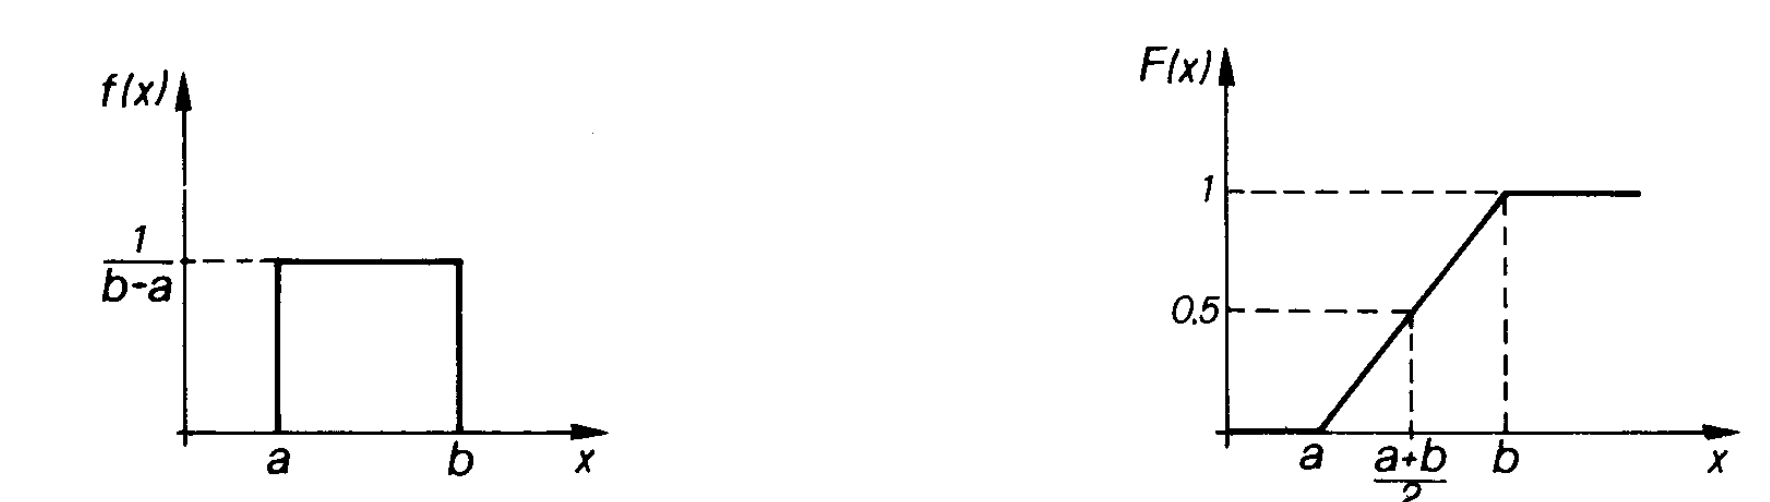
\includegraphics[scale=0.35]{../images/grafico_variabili_aleatorie_uniformi.png} 
\end{center}
% subsection Variabile aleatorie uniformi (end)

% subsection vari (end)